%Correct the file name.
%X: book number
%Y: part number
%ZZZ: page number in three digits. So page 3 would be 003.

\documentclass[11pt]{amsbook}

\usepackage{../HBSuerDemir}	% ------------------------


\begin{document}

% ++++++++++++++++++++++++++++++++++++++
\hPage{b1p1/193}
% ++++++++++++++++++++++++++++++++++++++
\noindent Let $ P(x_1)= \alpha_1 $ , \quad  $P(x_2)= \alpha_2$  \\
\indent $P''(x)= 6x-10  \Longrightarrow  P''(x_1)<0 , P''(x_2)>0 , P''(\frac{5}{3})=0 $ \\
\indent P(0)=8 \quad (y-intercept) \\
\indent $x^3 - 5x^2 + 2x + 8 =0 \Longrightarrow x_3=-1 \Longrightarrow x_4=2 , x_5=4 .$ (x-intercepts)
\indent $P(x)\rightarrow \infty  (-\infty) $ \quad as \quad $ x \rightarrow \infty (-\infty)$

\begin{figure}[htbp] 
\begin{center} 
\includegraphics[width=1.0\columnwidth]% 
{images/b1p1-193-fig01.png} 
\caption{ 
Covers of Calculus by Suer and Demir
}
\label{fig:SuerDemirCovers}
\end{center} 
\end{figure}

\indent Sketching the graph of a rational function: \\
\noindent Let \\
$$ R(x)= \frac{P(x)}{Q(x)} $$
be a rational function with \\
\indent $ P(x)= \sum_{k=0}^n a_k x^k $, \quad \quad  $Q(x)=b_k a^k$ 
\begin{hEnumerateArabic}
\item $D_R= \mathbb{R} - \hPairingCurly{ x: Q(x)=0 } $
\item $ Q(x)= 0$ gives vertical asymptotes at $x_i$' s  except $\lim_{x\to\ x_i} \frac{P(x)}{Q(x)} \not= \infty$
\item Asymptotes (other than vertical): \\
$y = 0$  is the horizontal asymptote if $n<m$,
\end{hEnumerateArabic}




%\begin{figure}[htb]
%	\centering
%	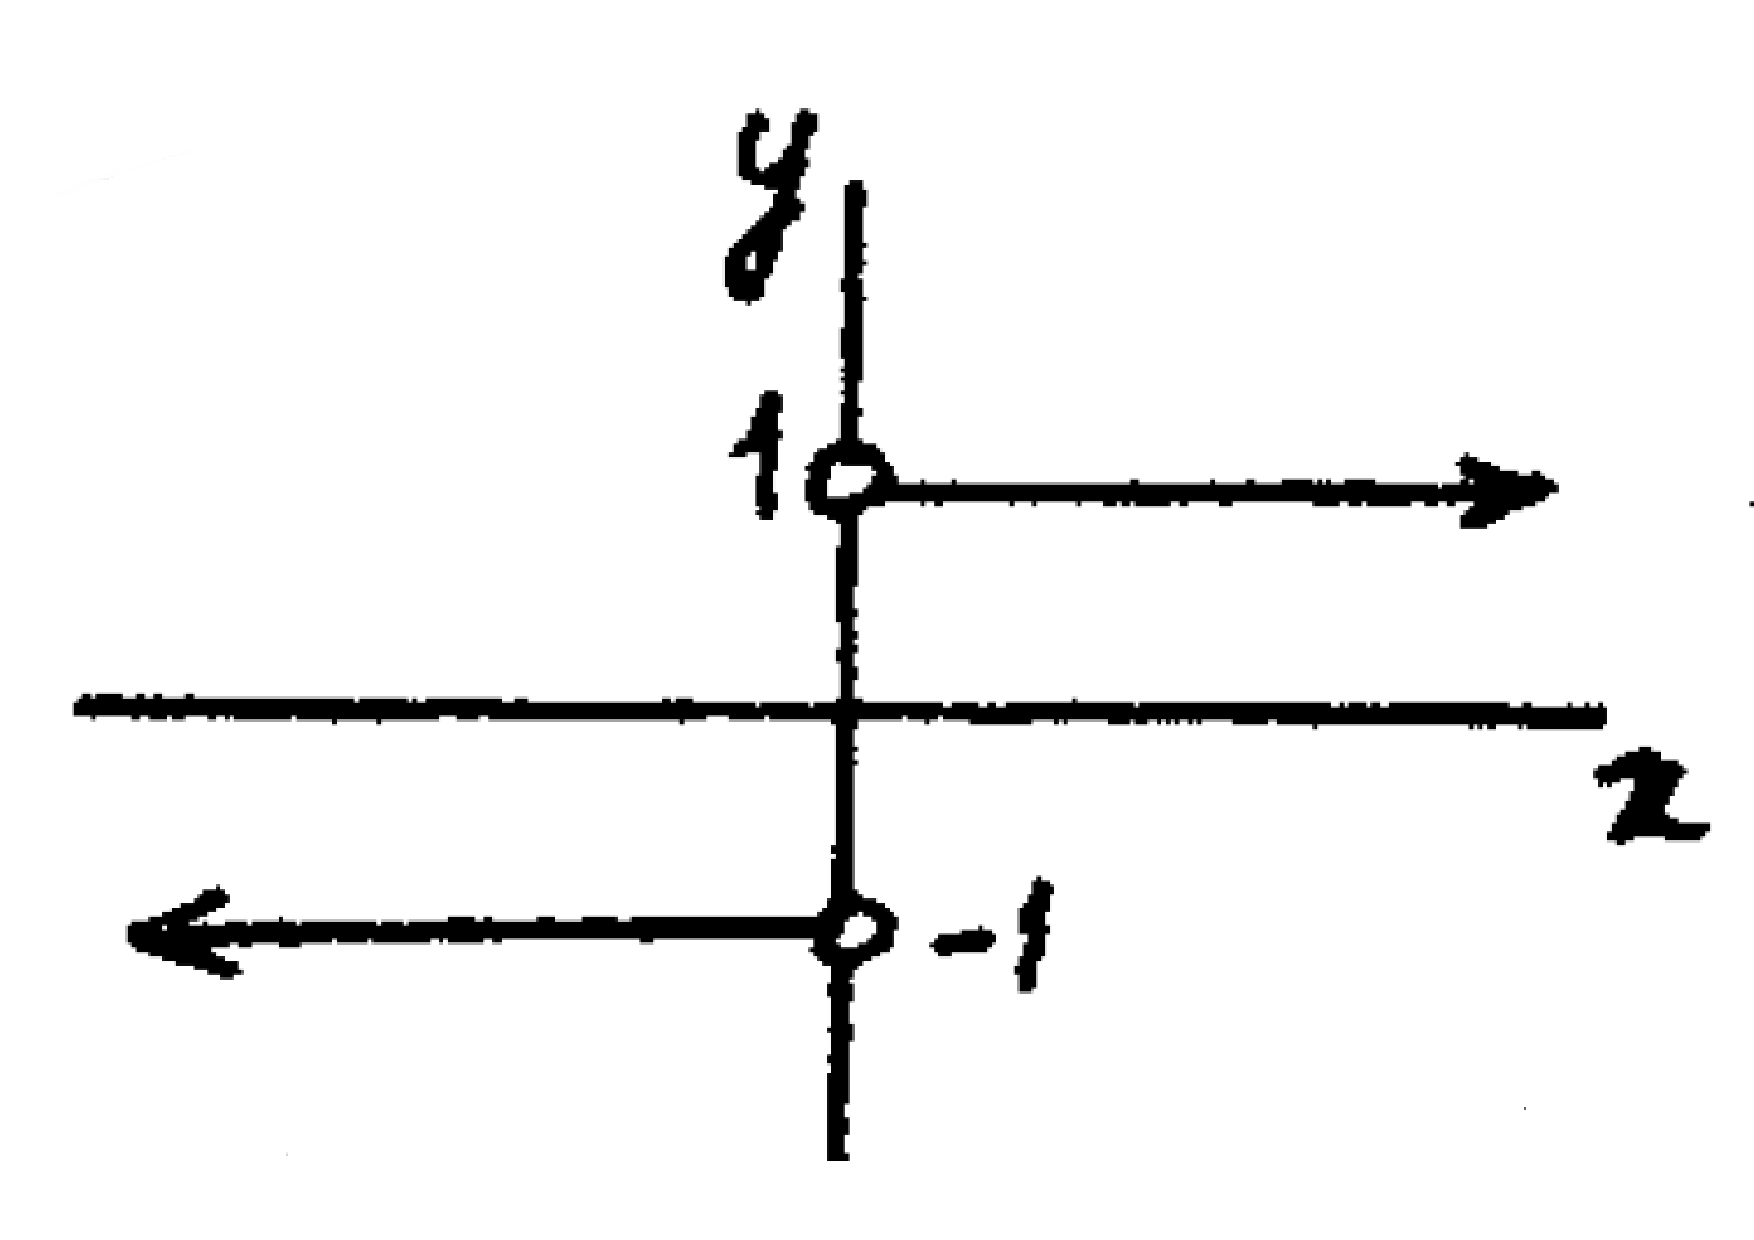
\includegraphics[width=0.45\textwidth]{images/bXpY-ZZZ-fig01}
%	\caption{Classification of complex numbers}
%	\label{fig:classificationOfComplexNumbersA}
%\end{figure}
%\begin{figure}[htb]
%	\centering
%	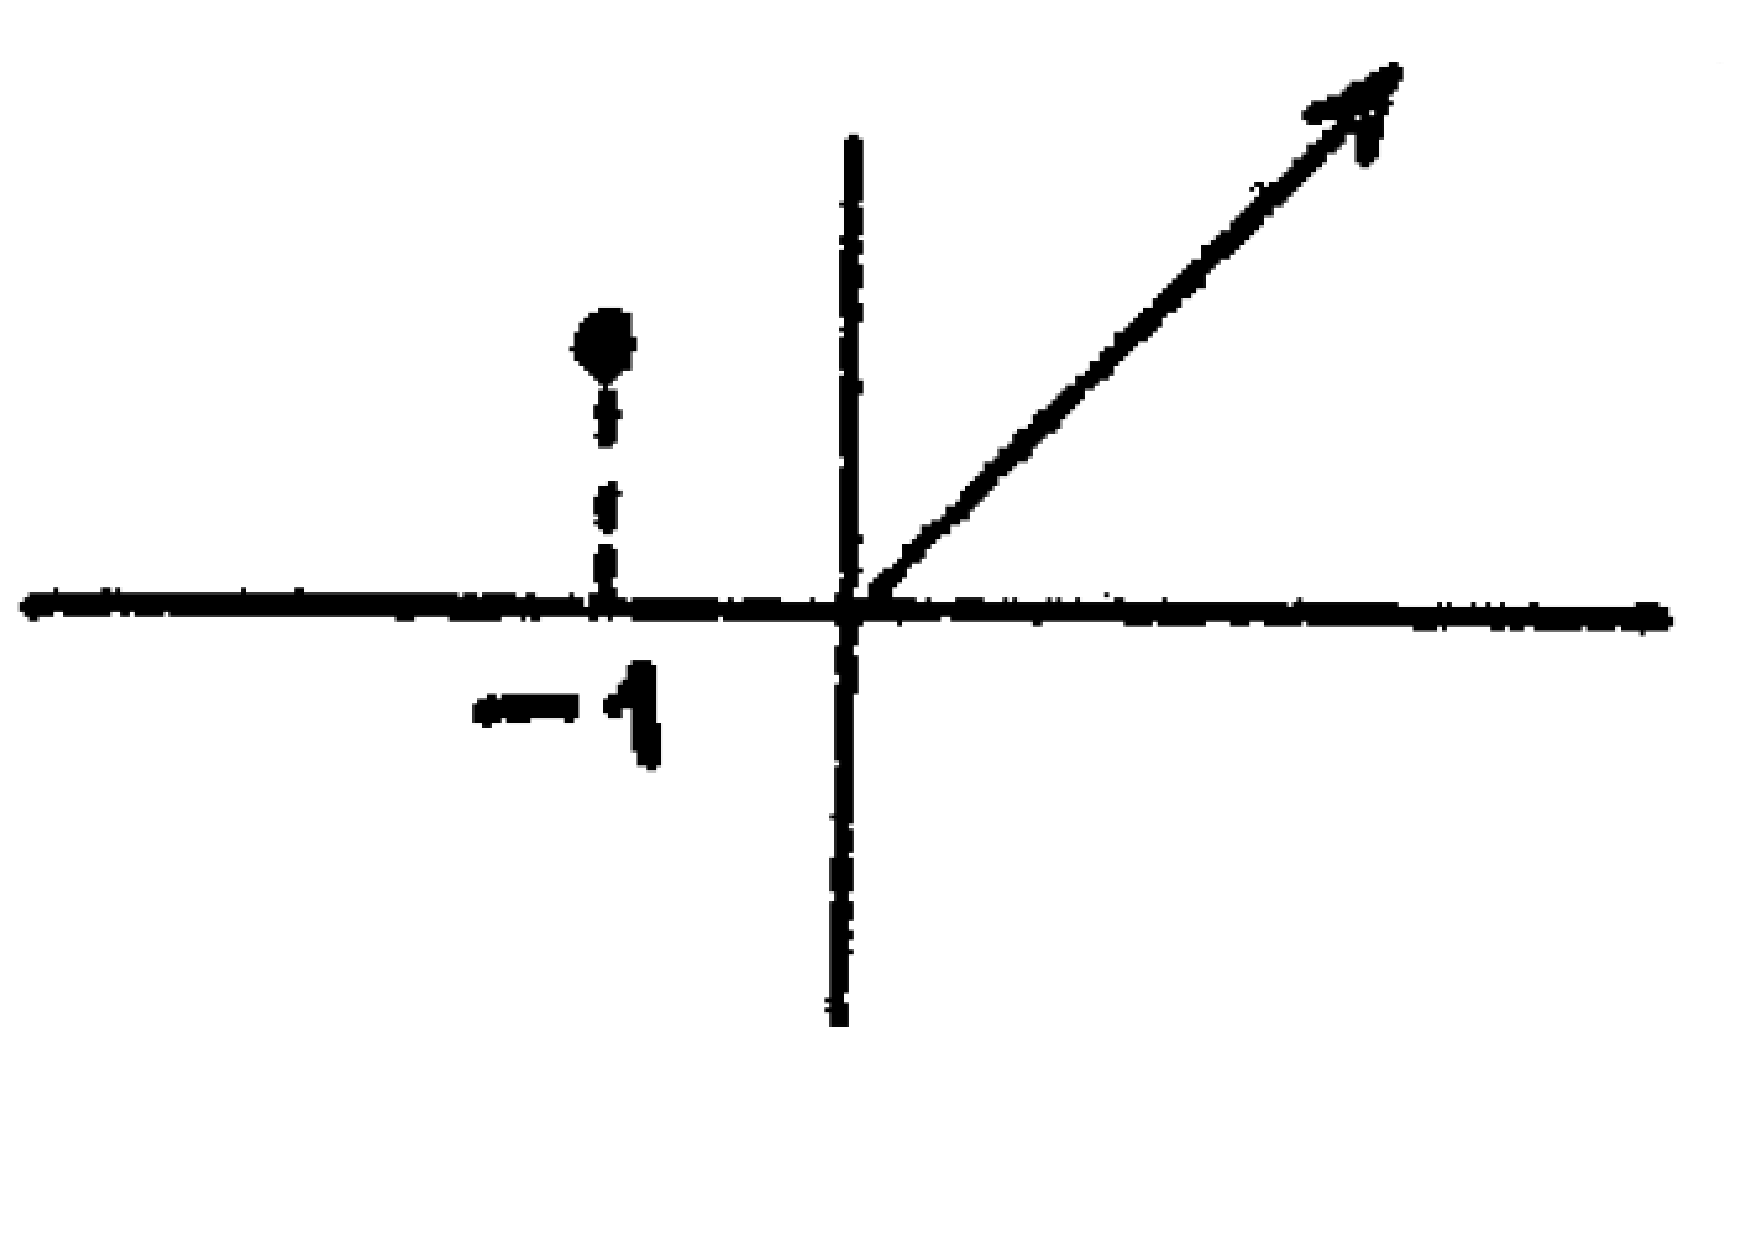
\includegraphics[width=0.45\textwidth]{images/bXpY-ZZZ-fig02}
%	\caption{Classification of complex numbers}
%	\label{fig:classificationOfComplexNumbersA}
%\end{figure}

% =======================================================
\end{document}  

%==== templates ====

%==== environments ====

%\begin{figure}[htb]
%	\centering
%	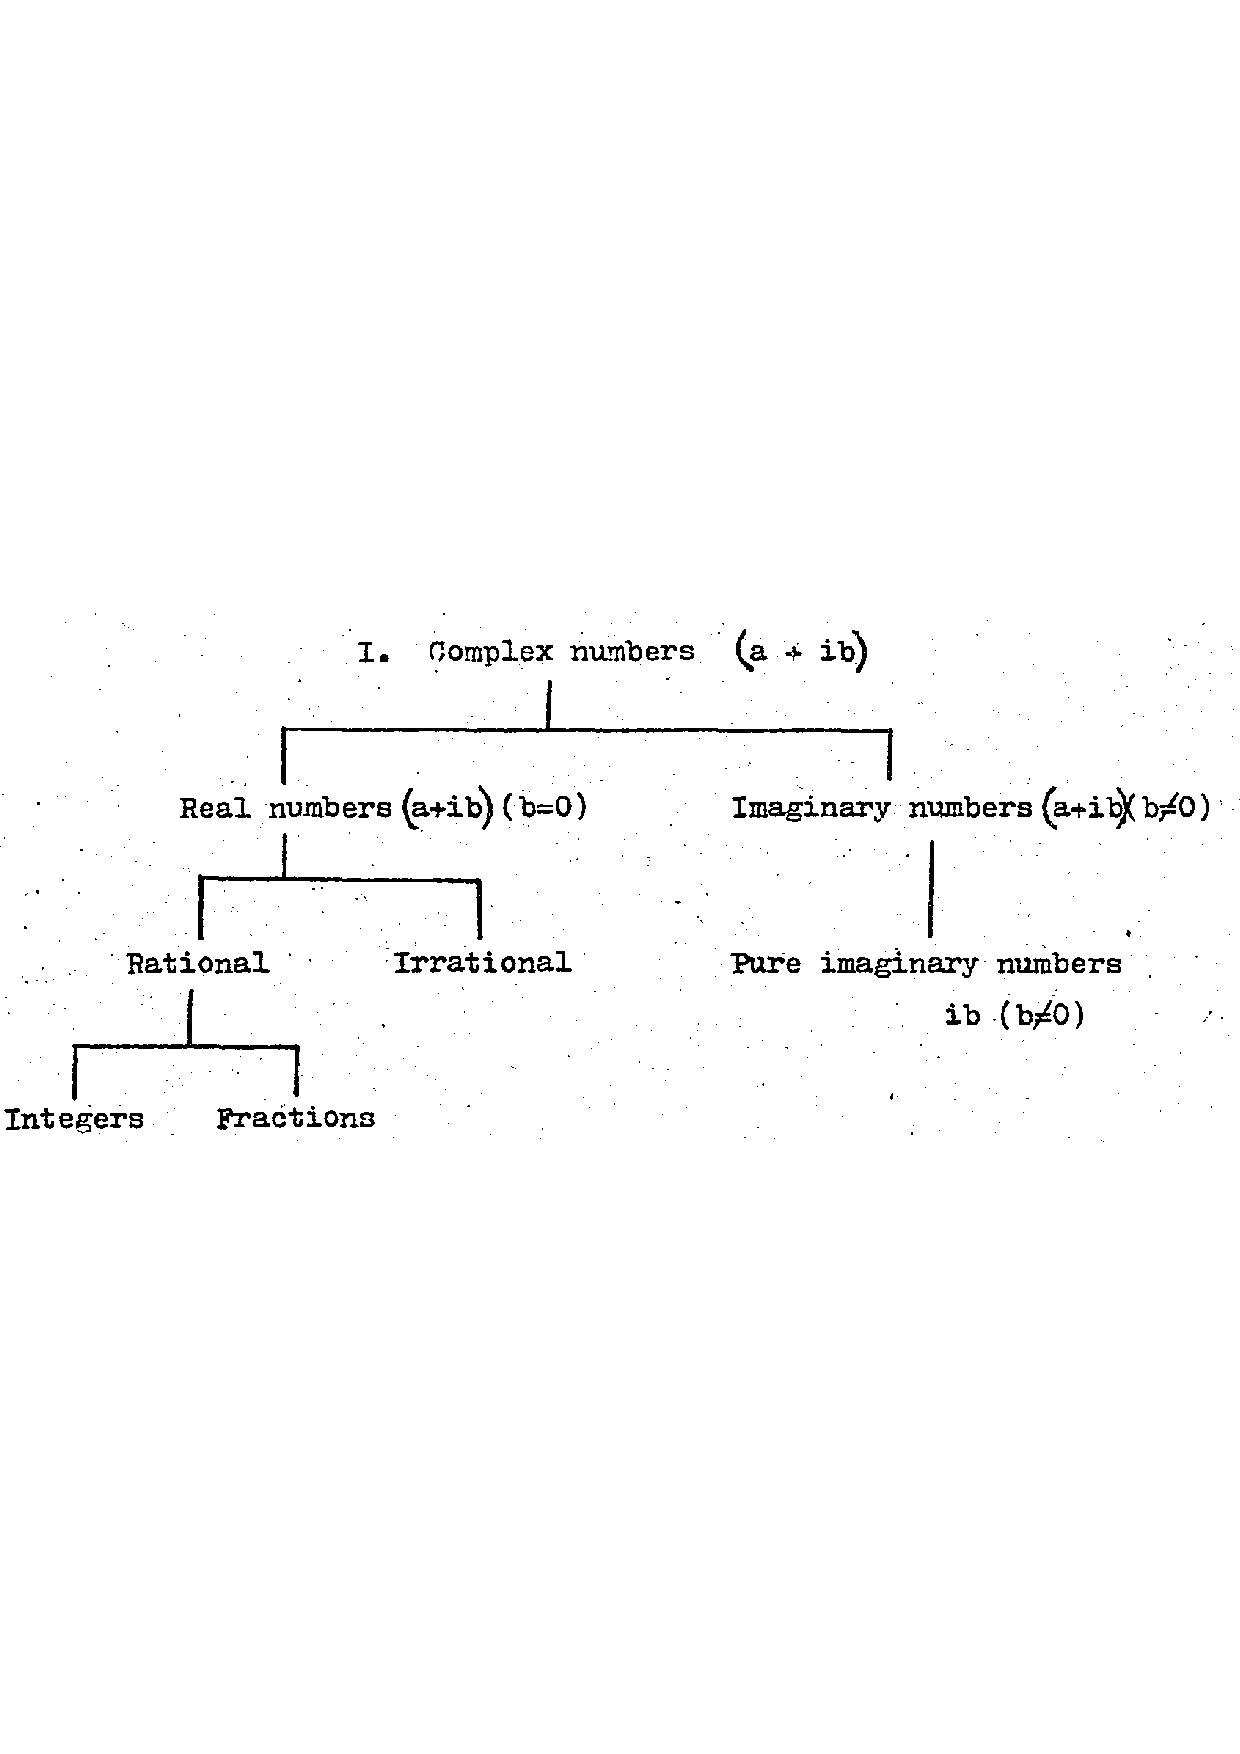
\includegraphics[width=0.9\textwidth]{images/SD-1-1p15A}
%	\caption{Classification of complex numbers}
%	\label{fig:classificationOfComplexNumbersA}
%\end{figure}

%\begin{center}
%\begin{tabular}{cc}
%\end{tabular}
%\end{center}

%\begin{exmp}
%\begin{hSolution}
%\end{hSolution}
%\end{exmp}

%\begin{hEnumerateAlpha}
%\end{hEnumerateAlpha}

%\begin{hEnumerateRoman}
%\end{hEnumerateRoman}

%$
%\begin{bmatrix}
%\end{bmatrix}
%$

%\frac{aaaa}{bbb}
%\frac{a_{n}}{b_{n}}
%\left( aaaa \right)
%\Longrightarrow

%\begin{multicols}{2}
%	bb
%\columnbreak
%	aa
%\end{multicols}
